\chapter{\vectorsInSpaceTitle}
\label{vectorsinspace}

%In vector calculus classes, you  encountered three-dimensional vectors.  Now we will develop the notion of $n$-vectors and learn some of their properties.
%
%\videoscriptlink{vectors_in_space_n_vectors_overview.mp4}{Overview}{scripts_vectors_in_space_n_vectors}

%We begin by looking at the space $\mathbb{R}^n$, which we can think of as the space of points with $n$ coordinates.  We then specify an \emph{origin} $O$, a favorite point in $\mathbb{R}^n$.  Now given any other point $P$, we can draw a \emph{vector} $v$ from $O$ to $P$.  Just as in $\mathbb{R}^3$, a vector has a \emph{magnitude} and a \emph{direction}.  
%
%\hypertarget{choosing_the_origin}{If} $O$ has coordinates $(o^1, \ldots, o^n)$ and $p$ has coordinates $(p^1, \ldots, p^n)$, then the \emph{components} of the vector $v$ are $\colvec{p^1 - o^1 \\ p^2- o^2 \\ \vdots \\ p^n - o^n }$.  This construction allows us to put the origin anywhere that seems most convenient in $\mathbb{R}^n$, not just at the point with zero coordinates:
%
%\begin{center}
%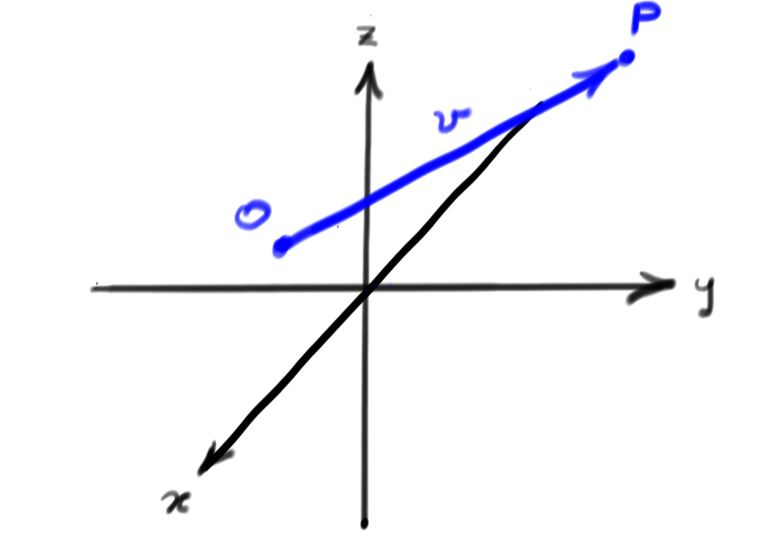
\includegraphics[scale =.3]{vectorOP.jpg}
%\end{center}

To continue our linear algebra journey, we must discuss $n$-vectors with an arbitrarily large number of components. 
The simplest way to think about these is as  ordered  lists of numbers, 
\[a=\ccolvec{a^1 \\ \vdots \\ a^n } .\]
%It is also convenient to think of n-vectors as functions with domain the set 
%$\{1,\dots,n\}$, as \hyperlink{vecs as fun}{discussed in chapter 1}. These two ideas give us the following two equivalent notions of the set of all $n$ vectors,
%\[
%{\mathbb{R}}^n =\left\{ \colvec{a^1 \\ \vdots \\ a^n } | \,  a^1,\dots a^n \in \mathbb{R} \right\}
%=\{ a:\{1,\dots,n\}\to \mathbb{R}\}
%\]
%
%Sometimes the notation $\mathbb{R}^{ \{1,\cdots,n\} }$ is used to emphasize the idea of functions from $   \{1,\cdots,n\} $ to $\mathbb{R}$.
\noindent
{\itshape 
Do not be confused by our use of a superscript to label components of a vector. Here $a^2$ denotes
the second component of the vector $a$, rather than the number $a$ squared!}  

\vspace{1mm}
We emphasize  that order matters: 
\begin{example} (Order of Components Matters)
\[\colvec{7 \\4 \\ 2\\ 5 } 
\neq \colvec{7 \\2 \\4 \\5 } .\]
\end{example}
The set of all $n$-vectors is denoted $\mathbb{R}^n$. As an equation
\[
{\mathbb{R}}^n :=\left\{ \colvec{a^1 \\ \vdots\ \  \\ a^n } \middle\vert \,  a^1,\dots, a^n \in \mathbb{R} \right\} \,.
\]
%; $2$-vectors and $3$-vectors are o

%\begin{remark}
%\hypertarget{note_points_versus_vectors}{A quick note on points versus vectors.} We might sometimes interpret a point and a vector as the same object, but they are slightly different concepts and should be treated as such. 
%%For more details, see \hyperref[points_vs_vectors]{Appendix~\ref*{points_vs_vectors}}
%\end{remark}


%\vspace{2mm}
%\noindent
%{\itshape 
%Do not be confused by our use of a superscript to label components of a vector. Here $v^2$ denotes
%the second component of a vector $v$, rather than a number $v$ squared!}  
%\vspace{4mm}

\section{Addition and Scalar Multiplication in ${\mathbb{R}}^n$}
A simple but important property of $n$-vectors is that we can {\itshape add} two $n$-vectors together and {\itshape multiply} one $n$-vector by a scalar:

\begin{definition} Given two $n$-vectors \(a\) and \(b\) whose components are given by 
\[a=\ccolvec{a^1 \\ \vdots  \\ a^n } \mbox{ and }\  b=\ccolvec{b^1 \\ \vdots  \\ b^n }\] their \emph{sum}\index{Vector addition!$n$-vectors} is \[a+b := \ccolvec{ a^1+b^1 \\ \vdots \\ a^n+b^n}\, .\]  
Given a scalar $\lambda$, the \emph{scalar multiple}\index{Scalar multiplication!$n$-vectors} \[\lambda a := \ccolvec{ \lambda a^1 \\ \vdots \\ \lambda a^n}\, .\]
\end{definition}

\begin{example}
Let 
\[a=\colvec{1\\2\\3\\4} \mbox{ and }\ b = \colvec{4\\3\\2\\1}\, .\]
Then, for example,
\[a+b= \colvec{5\\5\\5\\5} \mbox{ and }\  3a - 2b= \colvec{-5\\0\\5\\10}\, .\]
\end{example}

%Notice that these are the same rules we saw in \hyperref[vectoroperations]{Lecture 4}! 

%In Lectures 1-4, we thought of a vector as being a list of numbers which captured information about a linear system. Now we are thinking of a vector as a magnitude and a direction in \(\mathbb{R}^n,\) and luckily the same rules apply.

A special vector is the \emph{zero vector}\index{Zero vector!$n$-vectors}. 
%connecting the origin to itself.  
All of its components are zero:
\[
0=\ccolvec{0\\[-.5mm] \vdots \\ 0}=:0_n\, .
\]

In Euclidean geometry---the study of ${\mathbb R}^n$ with lengths and angles defined as in section~\ref{dirmag}
---$n$-vectors are used to label points  $P$ and the zero vector labels the origin $O$. In this sense,
  the zero vector is the only one  with zero magnitude, and the only one which points in no particular direction.  

\section{Hyperplanes}
Vectors in ${\mathbb R}^n$ are impossible to visualize unless $n$ is 1,2, or 3. However, familiar objects like lines and planes still make sense for any value of $n$:
The line $L$ along the direction defined by a vector $v$ and through a point $P$ labeled by a vector~$u$  can be written as 
\[L=\{ u + tv ~|~ t \in \mathbb{R} \}\, .\]  
Sometimes, since we know that a point $P$ corresponds to a vector,  we will be lazy and just write $L=\{P + tv ~|~ t \in \mathbb{R} \}$.  

\begin{example} %A line in ${\mathbb{R}}^4$.\\[.2cm]
$\left\{ \colvec{1\\2\\3\\4} + t\colvec{1\\0\\0\\0} \middle\vert t \in \mathbb{R} \right\}$ describes a line in ${\mathbb{R}}^4$ parallel to the $x_1$-axis.
\end{example}



%unrelated thought! 
%Any scalar multiple of a non-zero vector lies in the line determined by that vector.

Given two non-zero vectors $u,v$, they will \emph{usually} determine a plane, 
\begin{center}
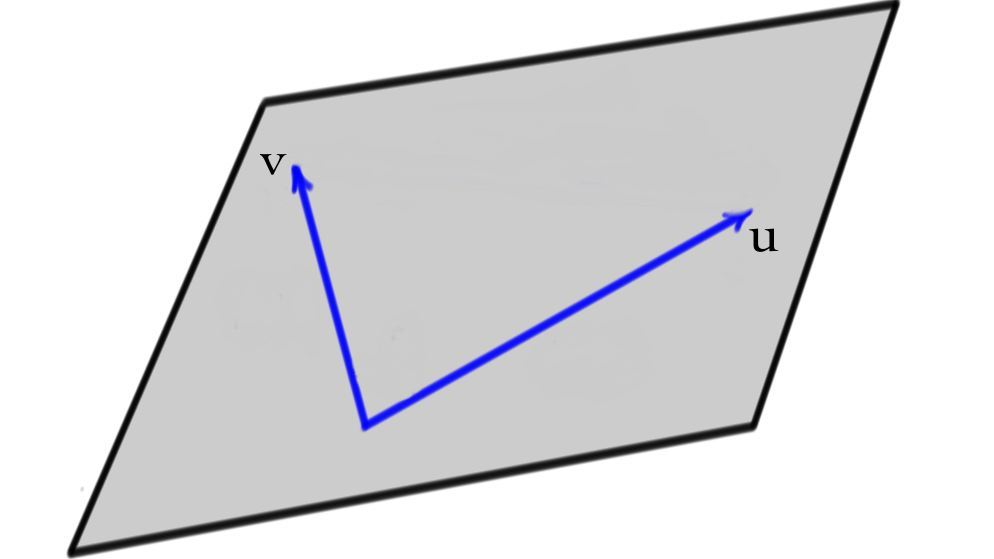
\includegraphics[alt={A plane in space with vectors u and v in the plane.},scale=.28]{uvplane.jpg}
\end{center}
unless both vectors are in the same line,  in which case, one of the vectors is a scalar multiple of the other.  The sum of $u$ and $v$ corresponds to laying the two vectors head-to-tail and drawing the connecting vector.  If $u$ and $v$ determine a plane, then their sum lies in the plane determined by $u$ and~$v$.
\begin{center}
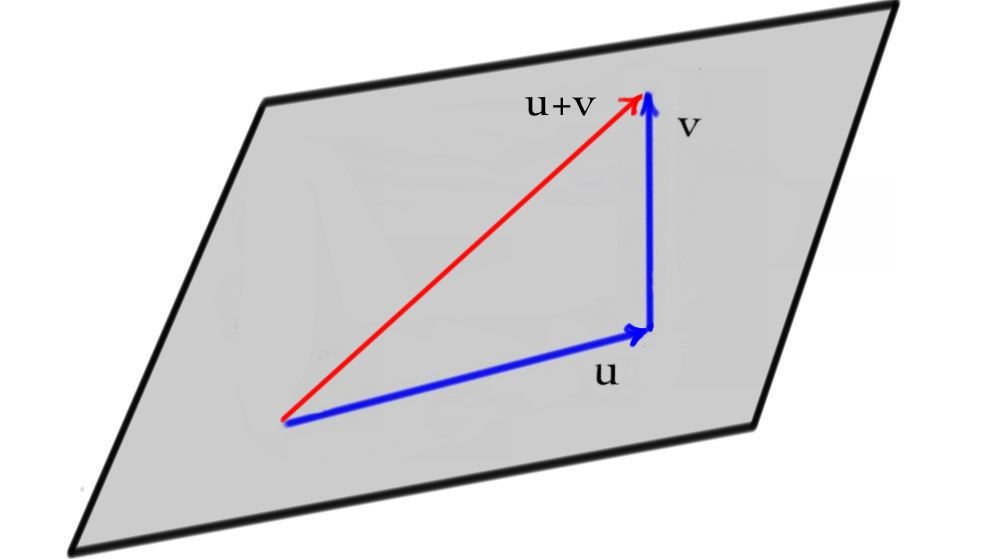
\includegraphics[alt={The same plane, but the vector v has been moved so that it starts where u ends.  The vector u+v goes from the start of u to the end of v.},scale=.28]{u+v.jpg}
\end{center}
The plane determined by two vectors $u$ and $v$ can be written as 
\[\{ P + su + tv ~|~ s, t \in \mathbb{R} \}\, .\]  


\begin{example}{(A plane in a higher dimensional space)} \label{2hyperplaneeg}
\[\left\{ \colvec{3\\1\\4\\1\\5\\9} + s\colvec{1\\0\\0\\0\\0\\0} + t\colvec{0\\1\\0\\0\\0\\0} \middle\vert s, t \in \mathbb{R} \right\}\] describes a plane in 6-dimensional space parallel to the $xy$-plane.
\end{example}

\Videoscriptlink{vectors_in_space_parametric.mp4}{Parametric Notation}{scripts_vectors_in_space_n_vectors_parametric}

\vspace{2mm}
We can generalize the notion of a plane with the following recursive definition. (That is, infinitely many things are defined in the following line.)

\begin{definition} A set of $k+1$ vectors $P,v_1, \ldots, v_k$ in $\mathbb{R}^n$ with $k\leq n$ determines a $k$-dimensional {\bfseries hyperplane}\index{Hyperplane}, 
\[
\left\{ P + \sum_{i=1}^{k} \lambda_iv_i\,  |\,  \lambda_i \in \mathbb{R} \right\}
\]
unless any of the vectors $v_j$ lives in the $(k-1)$-dimensional hyperplane determined by the other $k-1$ vectors
 \[
\left\{ 0 + \sum_{i\neq j}^{k} \lambda_iv_i\,  |\,  \lambda_i \in \mathbb{R} \right\}.
\]
%If the $k$ vectors do determine a $k$-dimensional hyperplane, then any point in the hyperplane can be written as:
\end{definition}


\begin{example}{(3+1 vectors that do not specify a  3-dimensional hyperplane)}
\[S:=\left\{ \colvec{3\\1\\4\\1\\5\\9} + s\colvec{1\\0\\0\\0\\0\\0} + t\colvec{0\\1\\0\\0\\0\\0} +u \colvec{1\\1\\0\\0\\0\\0}\middle\vert s, t,u \in \mathbb{R} \right\}\] 
is not a 3-dimensional hyperplane because 
\[\colvec{1\\1\\0\\0\\0\\0}=1\colvec{1\\0\\0\\0\\0\\0} + 1\colvec{0\\1\\0\\0\\0\\0} \in  \left\{     s\colvec{1\\0\\0\\0\\0\\0} + t\colvec{0\\1\\0\\0\\0\\0}  \middle\vert  s,t \in \mathbb{R} \right\}.\]
In fact, the set could be rewritten as 
\begin{align*}
S&=\left\{ \colvec{3\\1\\4\\1\\5\\9} + (s+u)\colvec{1\\0\\0\\0\\0\\0} + (t+u)\colvec{0\\1\\0\\0\\0\\0} \middle\vert s, t,u \in \mathbb{R} \right\}\\
&=
\left\{ \colvec{3\\1\\4\\1\\5\\9} + a\colvec{1\\0\\0\\0\\0\\0} + b\colvec{0\\1\\0\\0\\0\\0} \middle\vert a,b \in \mathbb{R} \right\}
\end{align*}
and so is actually the same 2-dimensional hyperplane in $\mathbb{R}^6$  as in example~\ref{2hyperplaneeg}.
\end{example}
















You might sometimes encounter the word ``hyperplane" without the qualifier ``k-dimensional. 
When the dimension $k$ is not specified, one usually assumes that $k=n-1$ for a hyperplane inside ${\mathbb R}^n$. This is the kind of object that is specified by one algebraic equation in $n$ variables. 

\begin{example}{(Specifying a plane with one linear algebraic equation.)}\\
The solution set to 
\[
x_1+x_2+x_3+x_4+x_5=1 \Leftrightarrow 
\colvec{x_1\\x_2\\x_3\\x_4\\x_5} =
\ccolvec{
1-x_2-x_3-x_4-x_5\\
\phantom{1-}x_2\phantom{-x_3-x_4-x_5}\\
\phantom{1-x_2-}x_3\phantom{-x_4-x_5}\\
\phantom{1-x_2-x_3-}x_4\phantom{-x_5}\\
\phantom{1-x_2-x_3-x_4-}x_5
}
\]
is
\[\left\{ \colvec{1\\0\\0\\0\\0} + 
s_2 \colvec{-1\\1\\0\\0\\0} + 
s_3 \colvec{-1\\0\\1\\0\\0} + 
s_4 \colvec{-1\\0\\0\\1\\0} + 
s_5 \colvec{-1\\1\\0\\0\\1}
\middle\vert s_2,s_3,s_4,s_5 \in \mathbb{R} \right\},\]
a 4-dimensional hyperplane in $\mathbb{R}^5$.
\end{example}


\section{Directions and Magnitudes}\label{dirmag}

Consider the {\itshape Euclidean length}\index{Euclidean length} of an $n$-vector: 
\[
\|v\| := \sqrt{(v^1)^2 + (v^2)^2+\cdots+(v^n)^2}\ =\ \sqrt{ \sum_{i=1}^n (v^i)^2 }\: .
\]
Using the Law of Cosines\index{Law of Cosines}, we can then figure out the angle between two vectors.  Given two vectors $v$ and $u$ that {\itshape span} a plane in $\mathbb{R}^n$, we can then connect the ends of $v$ and $u$ with the vector $v-u$. 
 \begin{center}
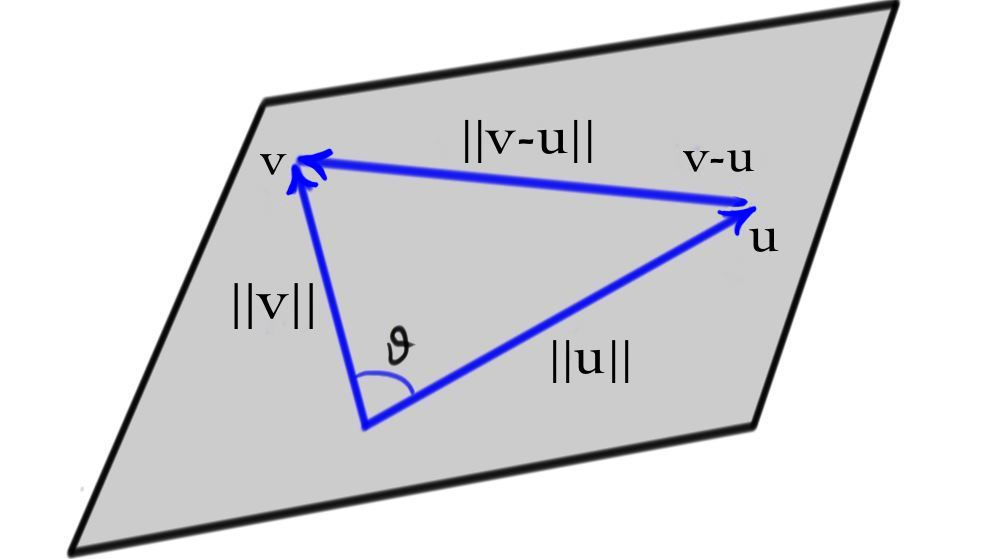
\includegraphics[alt={A plane with vectors u and v starting at the same point with angle θ between them.  The vector v-u points from the end of u to the end of v, making a triangle.  The sides of the triangle have lengths given by the lengths of the vectors.},scale=.24]{triangleineq.jpg}
\end{center}
Then the Law of Cosines states that:
\[ 
\|v-u\|^2 = \|u\|^2 + \|v\|^2 - 2\|u\|\,  \|v\| \cos \theta 
\]
Then isolate $\cos \theta$:
\begin{align*}
\|v-u\|^2 - \|u\|^2 - \|v\|^2
&= (v^1-u^1)^2 + \cdots + (v^n-u^n)^2 \\
& \quad - \big((u^1)^2 + \cdots + (u^n)^2\big) \\
& \quad - \big((v^1)^2 + \cdots + (v^n)^2\big) \\
& = -2 u^1v^1 - \cdots - 2u^nv^n
\end{align*}
Thus, 
\[
\|u\|\, \|v\| \cos \theta = u^1v^1 + \cdots + u^nv^n\, .
\]
Note that in the above discussion, we have assumed (correctly) that Euclidean lengths in ${\mathbb R}^n$
give the usual notion of lengths of vectors for any plane in ${\mathbb R}^n$. This now motivates the definition of the dot product.

\begin{definition} 
The {\bfseries dot product}\index{Dot product} of $u=\ccolvec{u^1 \\ \vdots \\ u^n }$ and $v=\ccolvec{v^1 \\ \vdots \\ v^n }$ is 
\[u\dotprod v := u^1v^1 + \cdots + u^nv^n\, .\]
\end{definition} 

\begin{example} of the dot product of two vectors from $\R^{100}$.
\[ \ccolvec{1\\2\\3\\4\\ \vdots \\ 100} \cdot 
\colvec{1\\1\\1\\1\\ \vdots \\ 1} = 1+2+3+\cdots+100=\frac12.100.101=5050.
\]
The sum above is the one Gau\ss, according to legend, could do in kindergarten\index{Kindergarten}.
\end{example}

\begin{definition} 
The {\bfseries length} (or {\bfseries norm} or {\bfseries magnitude}) of an n-vector\index{Length of a vector}\index{Norm|seealso{Length of a vector}}\index{Magnitude|seealso{Length of a vector}} $v$ is 
\[\|v\| := \sqrt{v\dotprod v }\, .\]
\end{definition} 

\begin{example} 
of the norm of a vector from $\R^{101}$.\\
\[\left\| \ccolvec{1\\2\\3\\4\\ \vdots \\ 101}\right\|
= 
\sqrt{\sum_{i=1}^{101} i^2} =   \sqrt{37,961}.
\]
\end{example}

\begin{definition} 
The {\bfseries angle}\index{Angle between vectors} $\theta$ between two vectors is determined by the formula \[u\dotprod v = \|u\|\|v\|\cos \theta\, .\]
\end{definition}

\begin{example} of an angle between two vectors form $\R^{101}$.\\
The angle between $ \ccolvec{1\\2\\3\\4\\ \vdots \\ 101} $ and 
$
\colvec{1\\0\\1\\0\\ \vdots \\ 1} $
is
$ 
\arccos  \left( \frac{10,201 }{\sqrt{37,916} \sqrt{51} } \right).
$
\end{example}




\begin{definition} 
Two vectors are \hypertarget{orthog}{{\bfseries orthogonal}}\index{Orthogonal} (or {\bfseries perpendicular}) if their dot product is zero.
\end{definition} 


\begin{example} of vectors from $\R^{101}$ that are orthogonal to each other.\\
\[
\colvec{1\\1\\1 \\ \vdots \\1} \cdot \colvec{1\\-1\\1\\ \vdots \\-1} =0.
\]
\end{example}

Notice that the zero vector $0_n$ from $\mathbb{R}^n$ is orthogonal to every vector in~$\mathbb{R}^n$; $0_n\cdot v=0$ for all $v \in \mathbb{R}^n$.

\vspace{2mm}\noindent
The dot product has some important properties; it is
\begin{enumerate}
\item  \emph{symmetric}:  
\[u\dotprod v = v\dotprod u\, ,\]
\item \emph{Distributive}:  \[u\dotprod (v+w) = u\dotprod v + u\dotprod w\, ,\]
\item \emph{Bilinear} (which is to say, linear in both $u$ and $v$):  
\[ u\dotprod (cv+dw) = c \, u\dotprod v +d \, u\dotprod w\, ,\] and 
\[(cu+dw)\dotprod v = c\, u\dotprod v + d\, w\dotprod v\, .\]
\item \emph{Positive Definite}: \[u\dotprod u \geq 0\, ,\] and  $u\dotprod u = 0$ only when $u$ itself is the $0$-vector.
\end{enumerate}

There are, in fact, many different useful ways to define lengths of vectors.  Notice in the definition above that we first defined the dot product, and then defined everything else in terms of the dot product.  So if we change our idea of the dot product, we change our notion of length and angle as well.  The dot product determines the \emph{Euclidean length and angle} between two vectors.  

Other definitions of length and angle arise from \index{Inner product}{\bfseries \hypertarget{inner_product}{inner products}}, which have all of the properties listed above
(except that in some contexts the positive definite requirement is relaxed). Instead of writing $\dotprod$ for other inner products, we usually write $\langle u,v \rangle$ to avoid confusion.

%\href{\webworkurl ReadingHomework5/1/}{Reading homework: problem 5.1}
\Reading{VectorsInSpace}{1}

\begin{example}\label{lorentzex}
Consider a four-dimensional space, with a special direction which we will call ``time''.  The \hypertarget{lorentzian_metric}{\emph{Lorentzian inner product}} on $\mathbb{R}^4$ is given by $\langle u,v \rangle = u^1v^1 + u^2v^2 + u^3v^3 - u^4v^4$.  This is of central importance in Einstein's theory of special relativity. Note, in particular,  that it is not positive definite.
As a result, the ``squared-length'' of a vector with coordinates $x, y, z$ and $t$ is $\|v\|^2 = x^2 + y^2 + z^2 - t^2$.  Notice that it is possible for $\|v\|^2\leq 0$ even with non-vanishing $v$!  
The physical interpretation of this inner product depends on the sign of the inner product; two space time points $X_1:=(x_1,y_1,z_1,t_1),~X_2:=(x_2,y_2,z_2,t_2)$  are 
\begin{itemize}
\item separated by a distance $\sqrt{ \langle X_1, X_2\rangle }$  if $\langle X_1, X_2\rangle \geq 0$.\\
\item separated by a time $\sqrt{ -\langle X_1, X_2\rangle }$  if $\langle X_1, X_2\rangle \leq 0.$
\end{itemize}
In particular, the difference in time coordinates $t_2-t_1$ is not the time between the two points! (Compare this to using polar coordinates for which the distance between two points $(r,\theta_1)$ and $(r,\theta_2)$ is not $\theta_2-\theta_1$; coordinate differences are not necessarily distances.)
\end{example}



\begin{theorem}[Cauchy-Schwarz Inequality]\index{Cauchy--Schwarz inequality}
For any non-zero vectors $u$ and~$v$ with an inner-product $\langle\:\  ,\:\,  \rangle$
\[ 
\frac{|\langle u,v \rangle|}{\|u\|\, \|v\|} \leq 1.
\]
\end{theorem}

The easiest proof would use the definition of the angle between two vectors and the fact that $\cos \theta \leq 1$. However, strictly speaking speaking we did not check our assumption that we could apply the Law of Cosines
to the Euclidean length in ${\mathbb R}^n$. There is, however a simple algebraic proof. 
\begin{proof}
Let $\alpha$ be any
real number and consider the following positive, quadratic polynomial in $\alpha$
\[
0\leq \langle u+\alpha v,u+\alpha v\rangle = \langle u,u\rangle +2\alpha \langle u,v\rangle +\alpha^2 \langle v,v\rangle\, .
\]
%(You should carefully check for yourself exactly which properties of an inner product were used to write down the above inequality! )
%Next, a tiny calculus computation shows that 
Since any quadratic $a\alpha^2 + 2b \alpha + c$ takes its minimal value
$c-\frac{b^2}{a}$
when $\alpha=-\frac{b}{2a}$,  and the inequality should hold for even this minimum value of the polynomial 
\[
0\leq \langle u,u\rangle -\frac{\langle u,v\rangle^2}{\langle v,v\rangle}\, 
\Leftrightarrow 
\frac{|\langle u,v \rangle|}{\|u\|\, \|v\|} \leq 1.\qedhere
\]
\end{proof}

\begin{theorem}[Triangle Inequality]\index{Triangle inequality}
For any $u,v\in \mathbb{R}^n$
\[ \|u+v\| \leq \|u\| + \|v\| .\]
\end{theorem}

\begin{proof}
We have
\begin{align*}
\|u+v\|^2 & = (u+v)\dotprod (u+v) \\
 	& = u\dotprod u + 2 u\dotprod v + v\dotprod v \\
	& = \|u\|^2 + \|v\|^2 + 2\,  \|u\|\,  \|v\| \cos \theta \\
	& = \left(\|u\| + \|v\|\right)^2 + 2 \, \|u\| \, \|v\| (\cos \theta -1) \\
	& \leq \left(\|u\| + \|v\|\right)^2	.
\end{align*}
That is, the square of the left-hand side of the triangle inequality is $\leq$ the square of the right-hand side. Since both the things being squared are positive, the inequality holds without the square;
\[ \|u+v\| \leq  \|u\| + \|v\|   \qedhere\]
\end{proof}

The triangle inequality is also ``self-evident'' when examining a sketch of $u$, $v$ and $u+v$.
\begin{center}
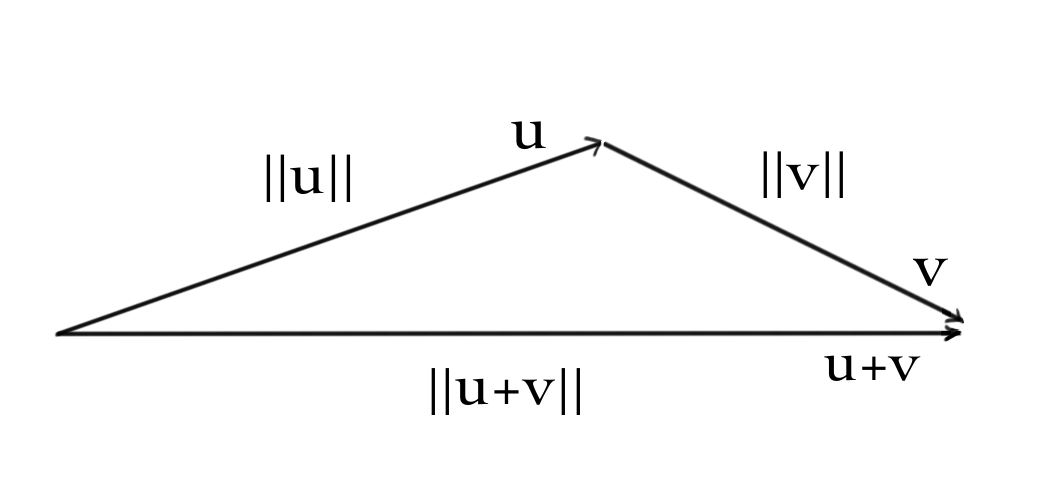
\includegraphics[alt={Vectors u and v, with v starting at the end of u.  The vector u+v goes from the beginning of u to the end of v, forming a triangle.  The sides of the triangle have lengths given by the lengths of the vectors.},scale=.25]{triangleagain.jpg}
\end{center}

\begin{example}
Let 
\[a=\colvec{1\\2\\3\\4} \mbox{ and }\ b = \colvec{4\\3\\2\\1}\, ,\]
so that
\begin{gather*}   a\dotprod a= b\dotprod b 
=1 +2^2+3^2+4^2=30 \\\Rightarrow \|a\|=\sqrt{30} =\| b \| \mbox{ and } \ 
\big(\|a\|+\|b\|\big)^2=(2\sqrt{30})^2=120\, .\end{gather*}
Since
\[a+b= \colvec{5\\5\\5\\5}\, , \quad \]
we have \[\|a+b\|^2=5^2+5^2+5^2+5^2=100<120=\big(\|a\|+\|b\|\big)^2\]
as predicted by the triangle inequality.

Notice also that $a\dotprod b=1.4+2.3+3.2+4.1=20< \sqrt{30}.\sqrt{30}=30=\|a\|\, \|b\|$ 
in accordance with the Cauchy--Schwarz inequality.
\end{example}

%\begin{center}\href{\webworkurl ReadingHomework5/2/}{Reading homework: problem 5.2}\end{center}
\Reading{VectorsInSpace}{2}


\section{Vectors, Lists and Functions: $\R^S$}
If you were  going shopping you might make something like the following list.

\begin{center}
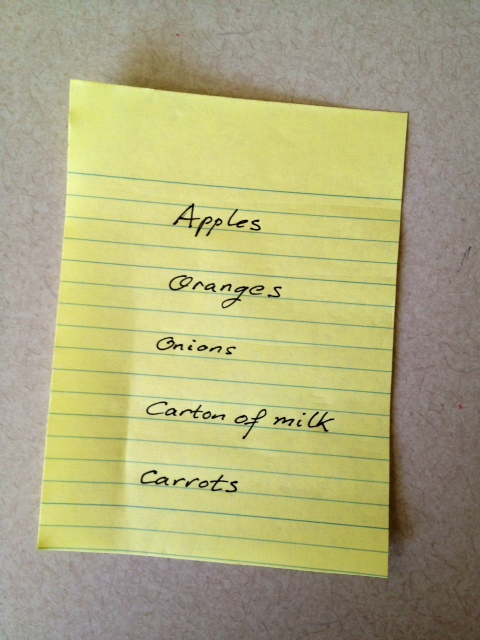
\includegraphics[alt={A shopping list with apples, oranges, onions, carton of milk, and carrots written on it.},scale =.3]{list.jpg}
\end{center}

\noindent
We could represent this information mathematically as a set, \[S=\{\text{apple, orange, onion, milk, carrot}\}\, .\] There is no information
of ordering here and no information about how many carrots you will buy. This set by itself is not a vector; how would we add such sets to 
one another?

If you were a more careful shopper your list might look like the following.

\begin{center}
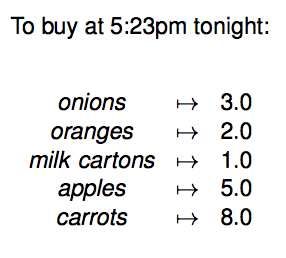
\includegraphics[alt={To buy at 5:23pm tonight: onions: 3.0, oranges: 2.0, milk cartons: 1.0, apples: 5.0, carrots: 8.0},scale =.5]{shoplist}
\end{center}

\noindent
What you have really done here is assign a number to each element of the set $S$. In other words, the second list is a function
\[
f:S\longrightarrow {\mathbb R}\, .
\]
Given two lists like the second one above, we could easily add them -- if you plan to buy 5 apples and I am buying 3 apples, together we
will buy 8 apples! In fact, the second list is really a 5-vector in disguise. 

In general
it is helpful to think of an $n$-vector as a function whose domain is the set 
$\{1,\dots,n\}$.
%, as \hyperlink{vecs as fun}{discussed in chapter 1}. 
This is equivalent to thinking of an $n$-vector as an ordered list of $n$ numbers.
These two ideas give us  two equivalent notions for the set of all $n$-vectors:
\[
{\mathbb{R}}^n :=\left\{ \ccolvec{a^1 \\ \vdots \\ a^n } \middle\vert \,  a^1,\dots ,a^n \in \mathbb{R} \right\}
=\{ a:\{1,\dots,n\}\to \mathbb{R}\} =: \mathbb{R}^{ \{1,\cdots,n\} }
\]
The notation $\mathbb{R}^{ \{1,\cdots,n\} }$ is used to denote the set of all functions from $   \{1,\dots,n\} $ to $\mathbb{R}$. 

Similarly, for any set $S$ the notation $\mathbb{R}^S$ denotes the set of functions from $S$ to~$\mathbb{R}$:
\[
{\mathbb R}^S:=\{ f:S\to {\mathbb R}\}\, .
\]
When $S$ is an ordered set like $\{1,\dots,n\}$, it is natural to write the components in order. When the elements of $S$ do not have a natural ordering, doing so might cause confusion. 



\begin{example}
{Consider the set } $S=\{*, \star, \# \}$ from \hyperlink{Consider the set}{chapter 1 review problem}~\ref{ch1rev}. A particular element of $\mathbb{R}^S$ is the function $a$ explicitly defined by 
\[ a^{\star}=3, a^{\#}=5, a^{*}=-2.\]
It is not natural to write 
\[
a=\colvec{3 \\ 5 \\ -2 } ~\text{or} ~a=\colvec{-2\\ 3 \\ 5 } 
\]
because the elements of $S$ do not have an ordering, since as sets $\{*, \star, \# \}=\{\star, \#,*\}$.
%, like the elements of $\{ 1,2,3\}$. 
\end{example}


In this important way, $\mathbb{R}^S$ seems different from $\mathbb{R}^3$. 
What is more evident are the similarities; since we can add two functions, we can add two elements of~$\mathbb{R}^S$:

\begin{example} Addition in $\mathbb{R}^{\{*, \star, \# \}}$\\
If $a,b \in \mathbb{R}^{\{*, \star, \# \}}$ 
such that 
\[a^{\star}=3, a^{\#}=5, a^{*}=-2\] 
and 
\[b^{\star}=-2, b^{\#}=4, b^{*}=13\]
then $a+b \in \mathbb{R}^S$ is the function such that
\[(a+b)^{\star}=3-2=1, (a+b)^{\#}=5+4=9, (a+b)^{*}=-2+13=11\, .\]
\end{example}

Also, since we can multiply functions by  numbers, there is a notion of scalar multiplication on $\mathbb{R}^S$.

\begin{example} Scalar Multiplication in $\mathbb{R}^S$\\
If $a \in \mathbb{R}^{\{*, \star, \# \}}$ such that
\[a^{\star}=3, a^{\#}=5, a^{*}=-2\]
then $3 a \in \mathbb{R}^{\{*, \star, \# \}}$ is the function such that 
\[(3a)^{\star}=3\cdot3=9, (3a)^{\#}=3\cdot5=15, (3a)^{*}=3(-2)=-6\, .\]

\end{example}

We visualize $\mathbb{R}^2$ and  $\mathbb{R}^3$ in terms of axes. We have a more abstract picture of  $\mathbb{R}^4$,  $\mathbb{R}^5$ and  $\mathbb{R}^n$ for larger $n$ while  $\mathbb{R}^S$ seems even more abstract. However, when thought of as a simple ``shopping list'',
you can see that vectors in $\mathbb{R}^S$ in fact, can describe everyday objects.
In chapter~\ref{vectorSpaces} we introduce the  general definition of a vector space that unifies all these different notions of a vector.

%\section*{References}
%
%Hefferon: Chapter One.II
%\\
%Beezer: Chapter V, Section VO, Subsection VEASM
%\\
%Beezer: Chapter V, Section O, Subsections IP-N
%\\
%Relevant Wikipedia Articles:
%\begin{itemize}
%\item \href{http://en.wikipedia.org/wiki/Dot_product}{Dot Product}
%\item \href{http://en.wikipedia.org/wiki/Inner_product_space}{Inner Product Space}
%\item \href{http://en.wikipedia.org/wiki/Minkowski_metric}{Minkowski Metric}
%\end{itemize} 


\section{Review Problems}

{\bfseries Webwork:} 
\begin{tabular}{|c|c|}
\hline
Reading problems &
\hwrref{VectorsInSpace}{1}, \hwrref{VectorsInSpace}{2}\\
Vector operations &  \hwref{VectorsInSpace}{3}\\
Vectors and lines &  \hwref{VectorsInSpace}{4}\\
Vectors and planes &\hwref{VectorsInSpace}{5}\\
Lines, planes and vectors & \hwref{VectorsInSpace}{6},\hwref{VectorsInSpace}{7}\\
Equation of a plane &\hwref{VectorsInSpace}{8},\hwref{VectorsInSpace}{9}\\
Angle between a line and plane &\hwref{VectorsInSpace}{10}
\\
\hline
\end{tabular}






\begin{enumerate}
\item \label{det33} Let $M=\begin{pmatrix}
m^1_1 & m^1_2 & m^1_3\\
m^2_1 & m^2_2 & m^2_3\\
m^3_1 & m^3_2 & m^3_3\\
\end{pmatrix}$.  Use row operations to put $M$ into \emph{row echelon form}.  For simplicity, assume that $m_1^1\neq 0 \neq m^1_1m^2_2-m^2_1m^1_2$.

Prove that $M$ is non-singular if and only if:
\[
m^1_1m^2_2m^3_3 
- m^1_1m^2_3m^3_2 
+ m^1_2m^2_3m^3_1 
- m^1_2m^2_1m^3_3 
+ m^1_3m^2_1m^3_2
- m^1_3m^2_2m^3_1
\neq 0
\]

\phantomnewpage

\item 
\begin{enumerate}
\item What does the matrix $E^1_2=\begin{pmatrix}
0 & 1 \\
1 & 0
\end{pmatrix}$ do to $M=\begin{pmatrix}
a & b \\
d & c
\end{pmatrix}$ under left multiplication?  What about right multiplication?
\item Find elementary matrices $R^1(\lambda)$ and $R^2(\lambda)$ that respectively multiply rows $1$ and $2$ of $M$ by $\lambda$ but otherwise leave $M$ the same under left multiplication.
\item Find a matrix $S^1_2(\lambda)$ that adds a multiple $\lambda$ of row $2$ to row $1$ under left multiplication.
\end{enumerate}

\phantomnewpage

\item Let $M$ be a matrix and $S^i_jM$ the same matrix with rows \(i\) and \(j\) switched.  Explain every line of the 
\hyperlink{rowswap}{series of equations} proving that $\det M = -\det (S^i_jM)$.

\phantomnewpage

%\item \label{prob_inversion_number} This problem is a ``hands-on'' look at why \hyperlink{permutation_parity}{the property} describing the parity of permutations is true.
%
%\hypertarget{inversion_number}{The \emph{inversion number}}\index{Permutation!Inversion number} of a permutation $\sigma$ is the number of pairs $i<j$ such that $\sigma(i)>\sigma(j)$; it's the number of ``numbers that appear left of smaller numbers'' in the permutation.  For example, for the permutation $\rho = [4,2,3,1]$, the inversion number is $5$. The number $4$ comes before $2,3,$ and $1$, and $2$ and $3$ both come before $1$.
%
%Given a permutation $\sigma$, we can make a new permutation $\tau_{i,j} \sigma$ by exchanging the $i$th and $j$th entries of $\sigma$.
%
%\begin{enumerate}
%\item What is the inversion number of the permutation \(\mu=[1,2,4,3]\) that exchanges 4 and 3 and leaves everything else alone? Is it an even or an odd permutation?
%
%\item What is the inversion number of the permutation \(\rho=[4,2,3,1]\) that exchanges 1 and 4 and leaves everything else alone? Is it an even or an odd permutation?
%
%\item What is the inversion number of the permutation \(\tau_{1,3} \mu\)? Compare the parity\footnote{The \emph{parity} of an integer refers to whether the integer is even or odd. Here the parity of a permutation $\mu$ refers to the parity of its inversion number.} of \(\mu\) to the parity of \(\tau_{1,3} \mu.\)
%
%\item What is the inversion number of the permutation \(\tau_{2,4} \rho\)? Compare the parity of \(\rho\) to the parity of \(\tau_{2,4} \rho.\)
%
%\item What is the inversion number of the permutation \(\tau_{3,4} \rho\)? Compare the parity of \(\rho\) to the parity of \(\tau_{3,4} \rho.\)
%\end{enumerate}
%
%\videoscriptlink{elementary_matrices_determinant_hint.mp4}{Problem~\ref{prob_inversion_number} hints}{scripts_elementary_matrices_determinants_hint}

\phantomnewpage

%\item \label{problem_permutation} (Extra credit) Here we will examine a (very) small set of the general properties about permutations and their applications. In particular, we will show that one way to compute the sign of a permutation is by finding the \hyperlink{inversion_number}{inversion number} $N$ of $\sigma$ and we have
%\[
%\sgn(\sigma) = (-1)^N.
%\]
%
%For this problem, let $\mu = [1,2,4,3]$.
%
%\begin{enumerate}
%\item Show that every permutation $\sigma$ can be sorted by only taking simple (adjacent) transpositions\index{Permutation!Simple transposition} $s_i$ where $s_i$ interchanges the numbers in position $i$ and $i+1$ of a permutation $\sigma$ (in our other notation $s_i = \tau_{i,i+1}$). For example $s_2 \mu = [1, 4, 2, 3]$, and to sort $\mu$ we have $s_3 \mu = [1, 2, 3, 4]$.
%
%\item \label{prob_part_relations} We can compose simple transpositions together to represent a permutation (note that the sequence of compositions is not unique), and these are associative, we have an identity (the trivial permutation where the list is in order or we do nothing on our list), and we have an inverse since it is clear that $s_i s_i \sigma = \sigma$. Thus permutations of $[n]$ under composition are an example of a \hyperref[groups]{group}. However note that not all simple transpositions commute with each other since
%\begin{align*}
%s_1 s_2 [1, 2, 3] & = s_1 [1, 3, 2] = [3, 1, 2]
%\\ s_2 s_1 [1, 2, 3] & = s_2 [2, 1, 3] = [2, 3, 1]
%\end{align*}
%(you will prove here when simple transpositions commute). When we consider our initial permutation to be the trivial permutation $e = [1, 2, \dotsc, n]$, we do not write it; for example $s_i \equiv s_i e$ and $\mu = s_3 \equiv s_3 e$. This is analogous to not writing 1 when multiplying. Show that $s_i s_i = e$ (in shorthand $s_i^2 = e$), $s_{i+1} s_i s_{i+1} = s_i s_{i+1} s_i$ for all $i$, and $s_i$ and $s_j$ commute for all $|i - j| \geq 2$.
%
%\item Show that every way of expressing $\sigma$ can be obtained from using the relations proved in part~\ref{prob_part_relations}. In other words, show that for any expression $w$ of simple transpositions representing the trivial permutation $e$, using the proved relations.
%
%\emph{Hint: Use induction on $n$. For the induction step, follow the path of the $(n+1)$-th strand by looking at $s_n s_{n-1} \cdots s_k s_{k\pm1} \cdots s_n$ and argue why you can write this as a subexpression for any expression of $e$. Consider using diagrams of these paths to help.}
%
%\item The simple transpositions \hyperlink{action}{acts on} an $n$-dimensional vector space $V$ by $s_i v = E^i_{i+1} v$ (where $E^i_j$ is \hyperlink{elem_matrix_row_swap}{an elementary matrix}) for all vectors $v \in V$. Therefore we can just represent a permutation $\sigma$ as the matrix $M_{\sigma}$\footnote{Often people will just use $\sigma$ for the matrix when the context is clear.}, and we have $\det(M_{s_i}) = \det(E^i_{i+1}) = -1$. Thus prove that $\det(M_{\sigma}) = (-1)^N$ where $N$ is a number of simple transpositions needed to represent $\sigma$ as a permutation. You can assume that $M_{s_i s_j} = M_{s_i} M_{s_j}$ (it is not hard to prove) and that $\det(A B) = \det(A) \det(B)$ \hyperref[detmultiplicative]{from Chapter~\ref*{elementarydeterminantsII}}.
%
%\emph{Hint: You to make sure $\det(M_{\sigma})$ is well-defined since there are infinite ways to represent $\sigma$ as simple transpositions.}
%
%\item Show that $s_{i+1} s_i s_{i+1} = \tau_{i, i+2}$, and so give one way of writing $\tau_{i, j}$ in terms of simple transpositions? Is $\tau_{i,j}$ an even or an odd permutation? What is $\det(M_{\tau_{i,j}})$? What is the inversion number of $\tau_{i,j}$?
%
%\item The minimal number of simple transpositions needed to express $\sigma$ is called the \emph{length}\index{Permutation!Length} of $\sigma$; for example the length of $\mu$ is 1 since $\mu = s_3$. Show that the length of $\sigma$ is equal to the inversion number of $\sigma$.
%
%\emph{Hint: Find an procedure which gives you a new permutation $\sigma^{\prime}$ where $\sigma = s_i \sigma^{\prime}$ for some $i$ and the inversion number for $\sigma^{\prime}$ is 1 less than the inversion number for $\sigma$.}
%
%\item Show that $(-1)^N = \sgn(\sigma) = \det(M_{\sigma})$, where $\sigma$ is a permutation with $N$ inversions. Note that this immediately implies that $\sgn(\sigma \rho) = \sgn(\sigma) \sgn(\rho)$ for any permutations $\sigma$ and $\rho$.
%\end{enumerate}

\item Let $M'$ be the matrix obtained from $M$ by swapping two columns $i$ and $j$. Show that $\det M'=-\det M $.

\item The scalar triple product of three vectors $u,v,w$ from $\Re^3$ is $u\cdot(v\times w)$. Show that this product is the same as the determinant of the matrix whose columns are $u,v,w$ (in that order). What happens to the scalar triple product when the factors are permuted? 

\item Show that if $M$ is a $3\times 3$ matrix whose third row is a sum of multiples of the other rows ($R_3=aR_2+bR_1$) then $\det M=0$. Show that the same is true if one of the columns is a sum of multiples of the others. 

\end{enumerate}

\phantomnewpage

\newpage
